\documentclass{article}
\newenvironment{standalone}{\begin{preview}}{\end{preview}}
\usepackage{../includes}

\begin{document}
\begin{standalone}
  \section{Introducción}

  \subsection{Arreglo de antenas} \label{subsec:arreglo}

  Un arreglo de antenas es un conjunto de elementos o radiadores.
  Una de las ventajas de usar un arreglo de antenas en lugar de una antena directiva es que mediante cambios en las fases entre los elementos del arreglo, sumadas a las diferencias de fases debidas a las diferentes posiciones de los elementos en el arreglo, se puede obtener máxima radiación en una dirección deseada.
  Esto se conoce como apuntamiento de haz \cite{visser2005}.

  Existen diversas geometrías que un arreglo de antenas puede tomar.
  En este trabajo, estudiaremos la más simple, un arreglo lineal de antenas.
  En éste, los elementos están ubicados sobre un eje, llamada apertura del arreglo.
  El eje perpendicular a la apertura del arreglo se llama normal del arreglo y un punto sobre esta línea, por encima del arreglo, se denomina cénit.
  Por conveniencia, aunque no es necesario, se considera que los radiadores son iguales y que se encuentran equiespaciados.

  Cuando el arreglo de antenas recibe un frente de ondas, podemos definir el ángulo $\theta$ que forma el frente de ondas con la apertura del arreglo, o la dirección de la radiación con la normal del arreglo, como se muestra en la \cref{fig:arreglo-antenas}.

  \begin{figure}[!htbp]
    \centering
    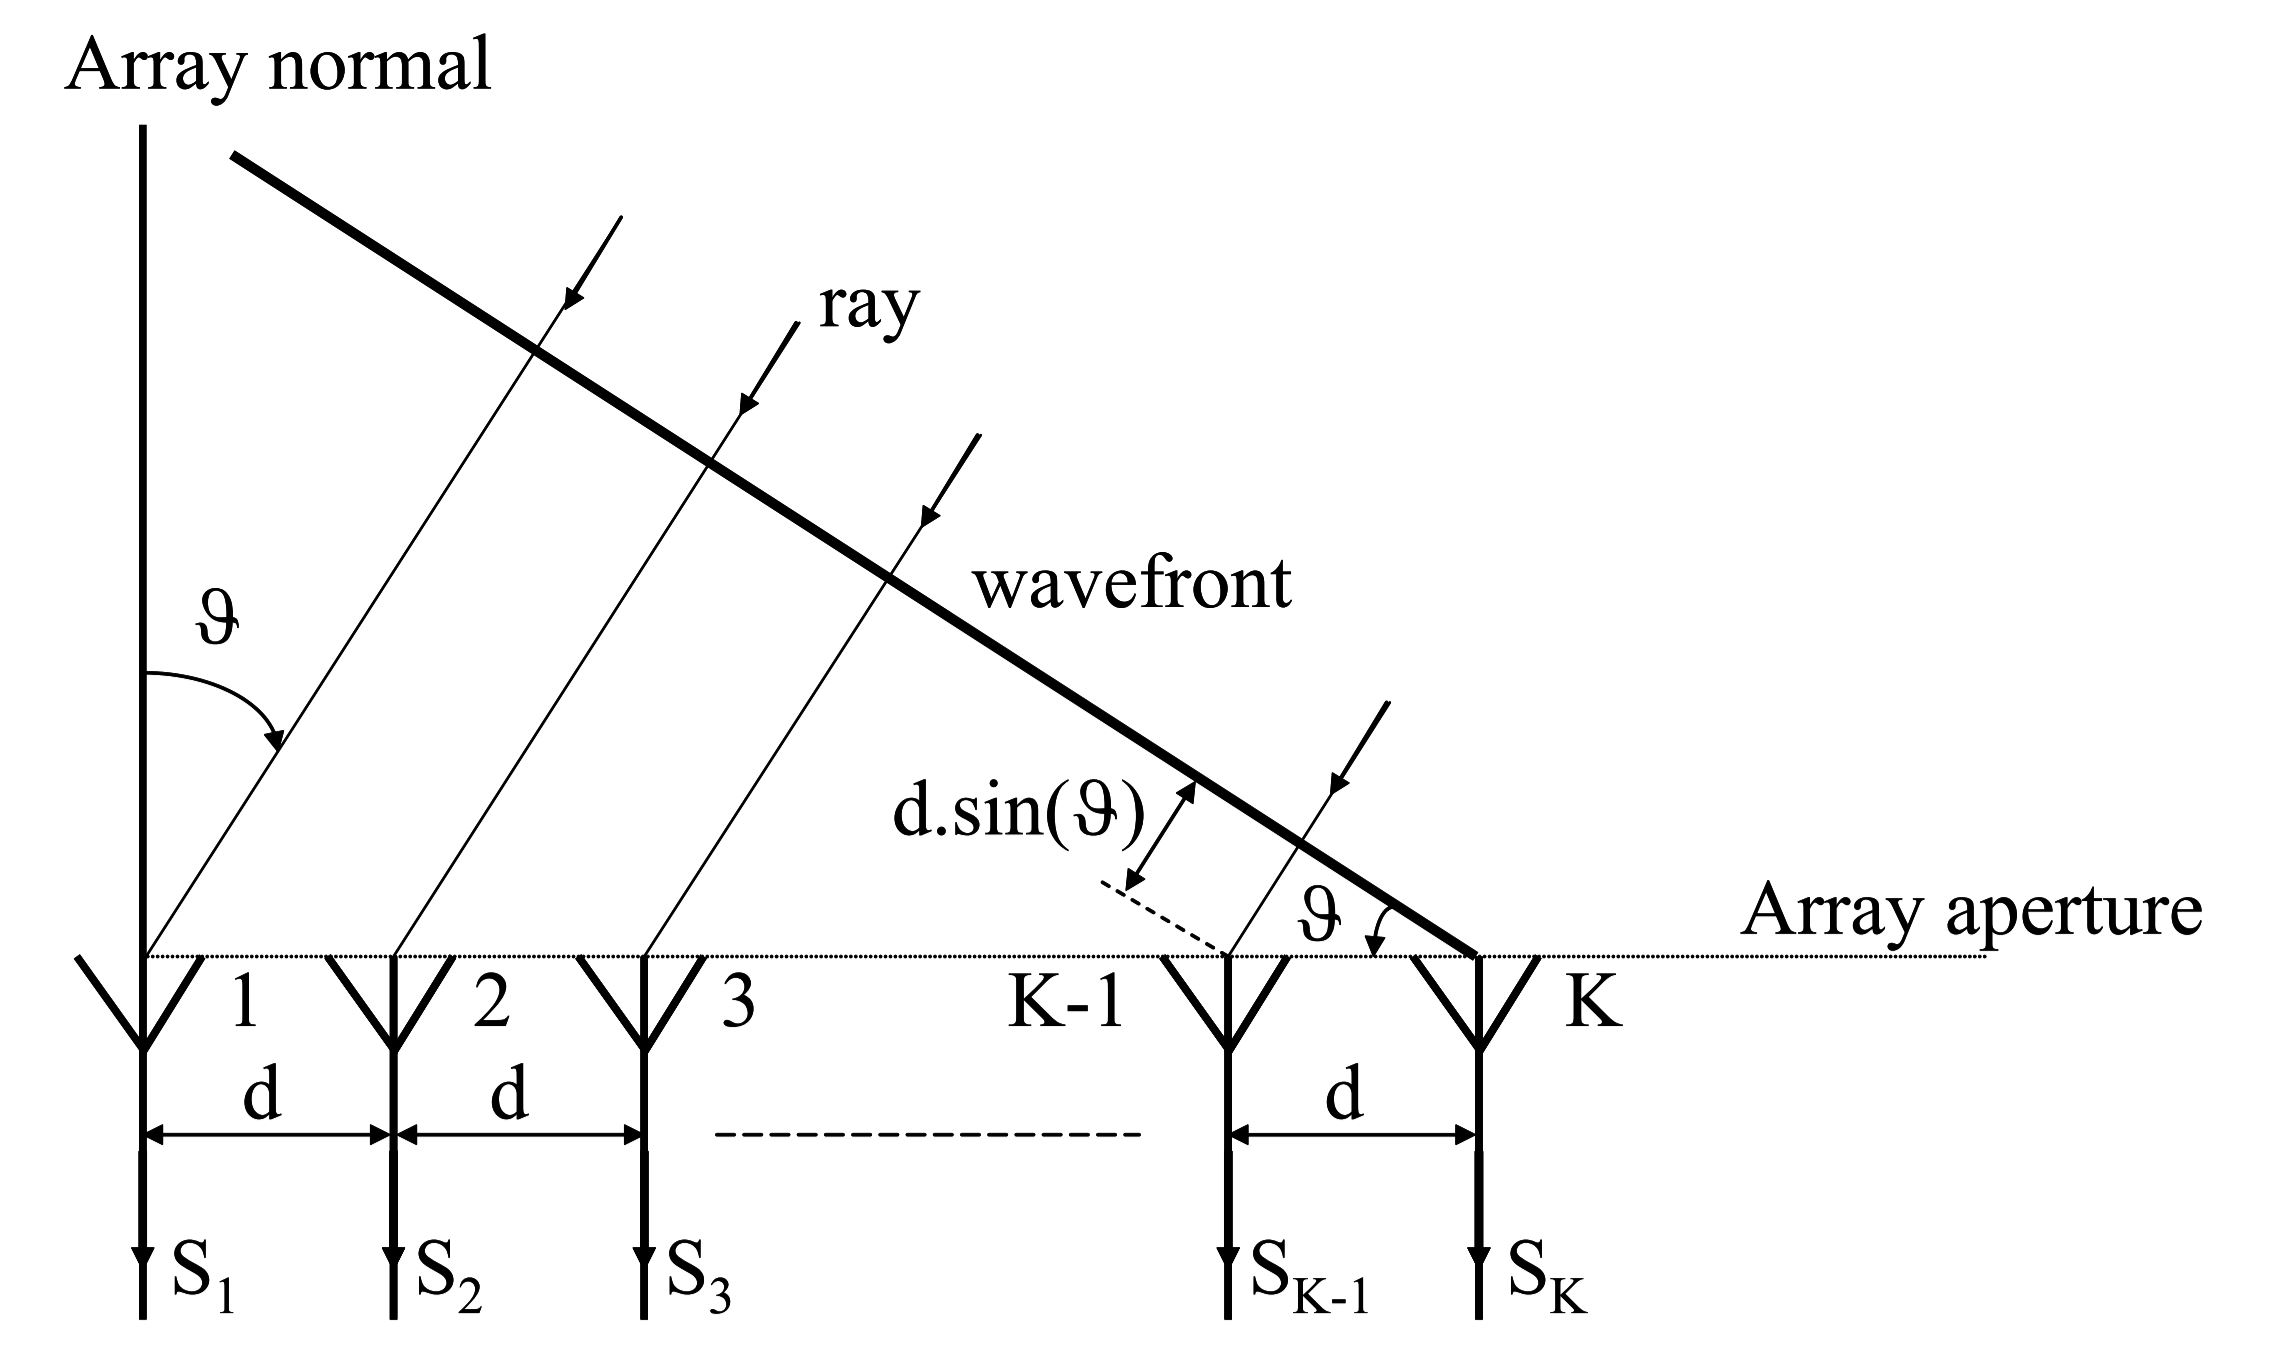
\includegraphics[width=\linewidth, height=50mm, keepaspectratio]{arreglo-antenas.jpg}
    \caption{Arreglo lineal de antenas, extraído de \cite{visser2005}.}
    \label{fig:arreglo-antenas}
  \end{figure}

  Puede verse que, dependiendo del ángulo $\theta$, las señales recibidas por cada elemento del arreglo estarán desfasadas.
  Al sumar estas señales, se generarán interferencias constructivas y destructivas dependientes de este desfasaje.
  Si no añadimos ningún retraso adicional, las señales son máximas en la dirección de la normal del arreglo.
  Podemos observar este fenómeno en lo que se denomina patrón de radiación del arreglo, como se muestra en la \cref{fig:patron-radiacion-sin-apuntamiento}.
  El patrón de radiación de un arreglo lineal de antenas consta de un lóbulo principal de máxima ganancia y algunos lóbulos secundarios donde la ganancia es menor y zonas de anulación en donde la interferencia destructiva es total.

  \begin{figure}[!htbp]
    \centering
    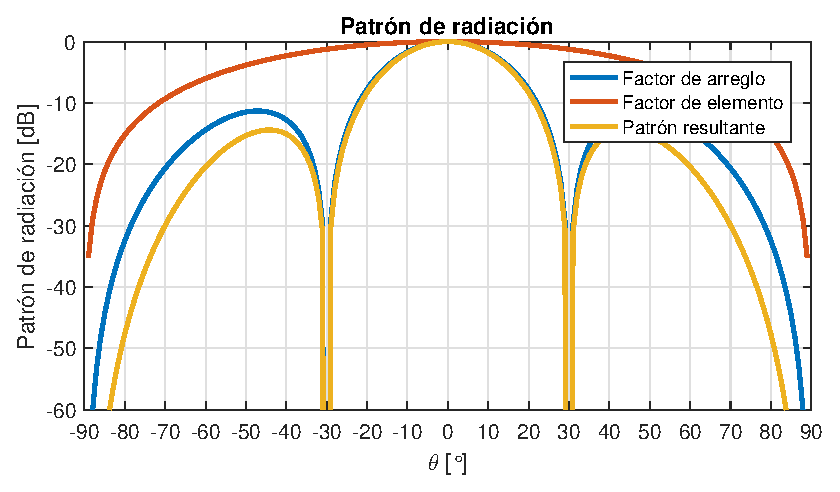
\includegraphics[width=\linewidth, height=60mm, keepaspectratio]{radiation-pattern-broadside.eps}
    \caption{Patrón de radiación de un arreglo de antena sin apuntamiento de haz.}
    \label{fig:patron-radiacion-sin-apuntamiento}
  \end{figure}

  Si añadimos un desfasaje adicional en las señales, el lóbulo principal se moverá y estaremos realizando un apuntamiento de haz como se muestra en la \cref{fig:patron-radiacion-con-apuntamiento}.

  \begin{figure}[!htbp]
    \centering
    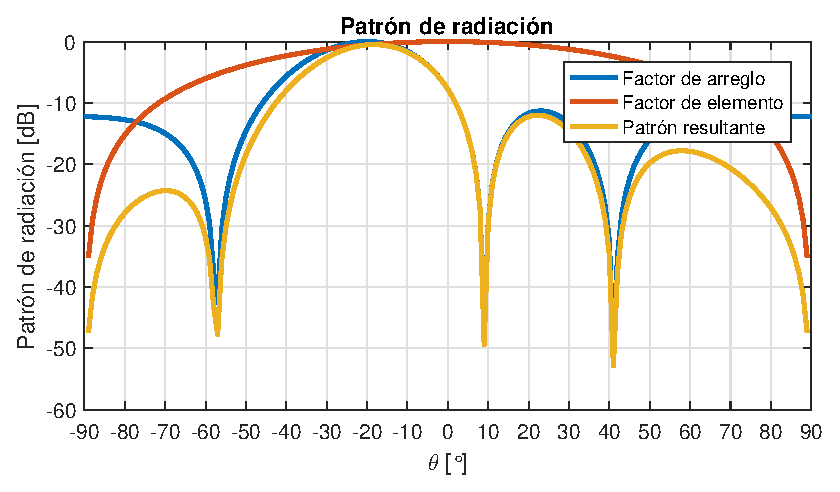
\includegraphics[width=\linewidth, height=60mm, keepaspectratio]{radiation-pattern-beamforming.eps}
    \caption{Patrón de radiación de un arreglo de antena con apuntamiento de haz en $\theta = -20\degree$.}
    \label{fig:patron-radiacion-con-apuntamiento}
  \end{figure}

  \subsection{Síntesis digital directa} \label{subsec:dds}

  La síntesis digital directa, o DDS por sus siglas en inglés (\textit{Direct Digital Synthesis}), es un método para producir señales analógicas mediante la generación de una señal digital y la posterior conversión analógica-digital \cite{murphy2004}.

  La \cref{fig:componentes-dds} muestra los componentes básicos de un sintetizador.
  El acumulador de fase representa la fase, un ángulo, de la señal a generar.
  El conversor de fase a amplitud entrega el seno de dicho ángulo.

  \begin{figure}[!htbp]
    \centering
    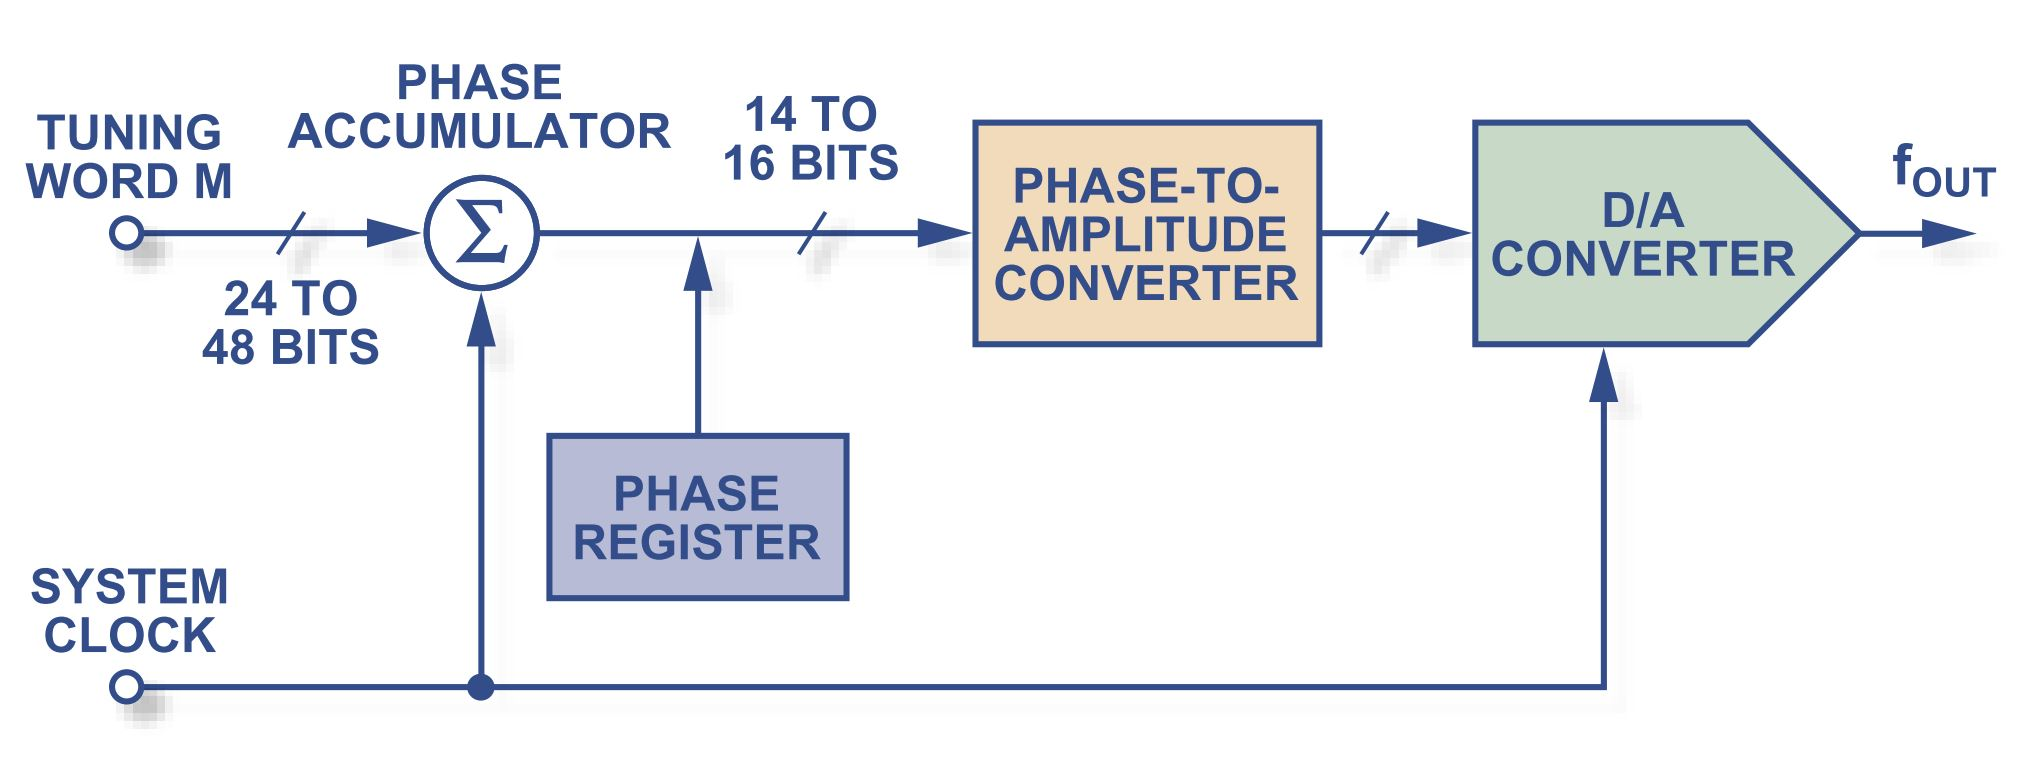
\includegraphics[width=\linewidth, height=40mm, keepaspectratio]{componentes-dds.jpg}
    \caption{Componentes de un sintetizador digital directo, extraído de \cite{murphy2004}.}
    \label{fig:componentes-dds}
  \end{figure}

  El conversor de fase a amplitud es usualmente una \textit{look-up table}, es decir una tabla con los valores de una función.
  En este caso, la función seno.
  La frecuencia generada dependerá entonces de la frecuencia del reloj del sistema y de la palabra de ajuste de frecuencia M.
  Esta palabra representa los saltos que se dan al recorrer la \textit{look-up table}.
  Mientras más grandes sean estos saltos, más rápido se recorrerá la tabla y mayor será la frecuencia de salida como se ilustra en la \cref{fig:look-up-table}.

  \begin{figure}[!htbp]
    \centering
    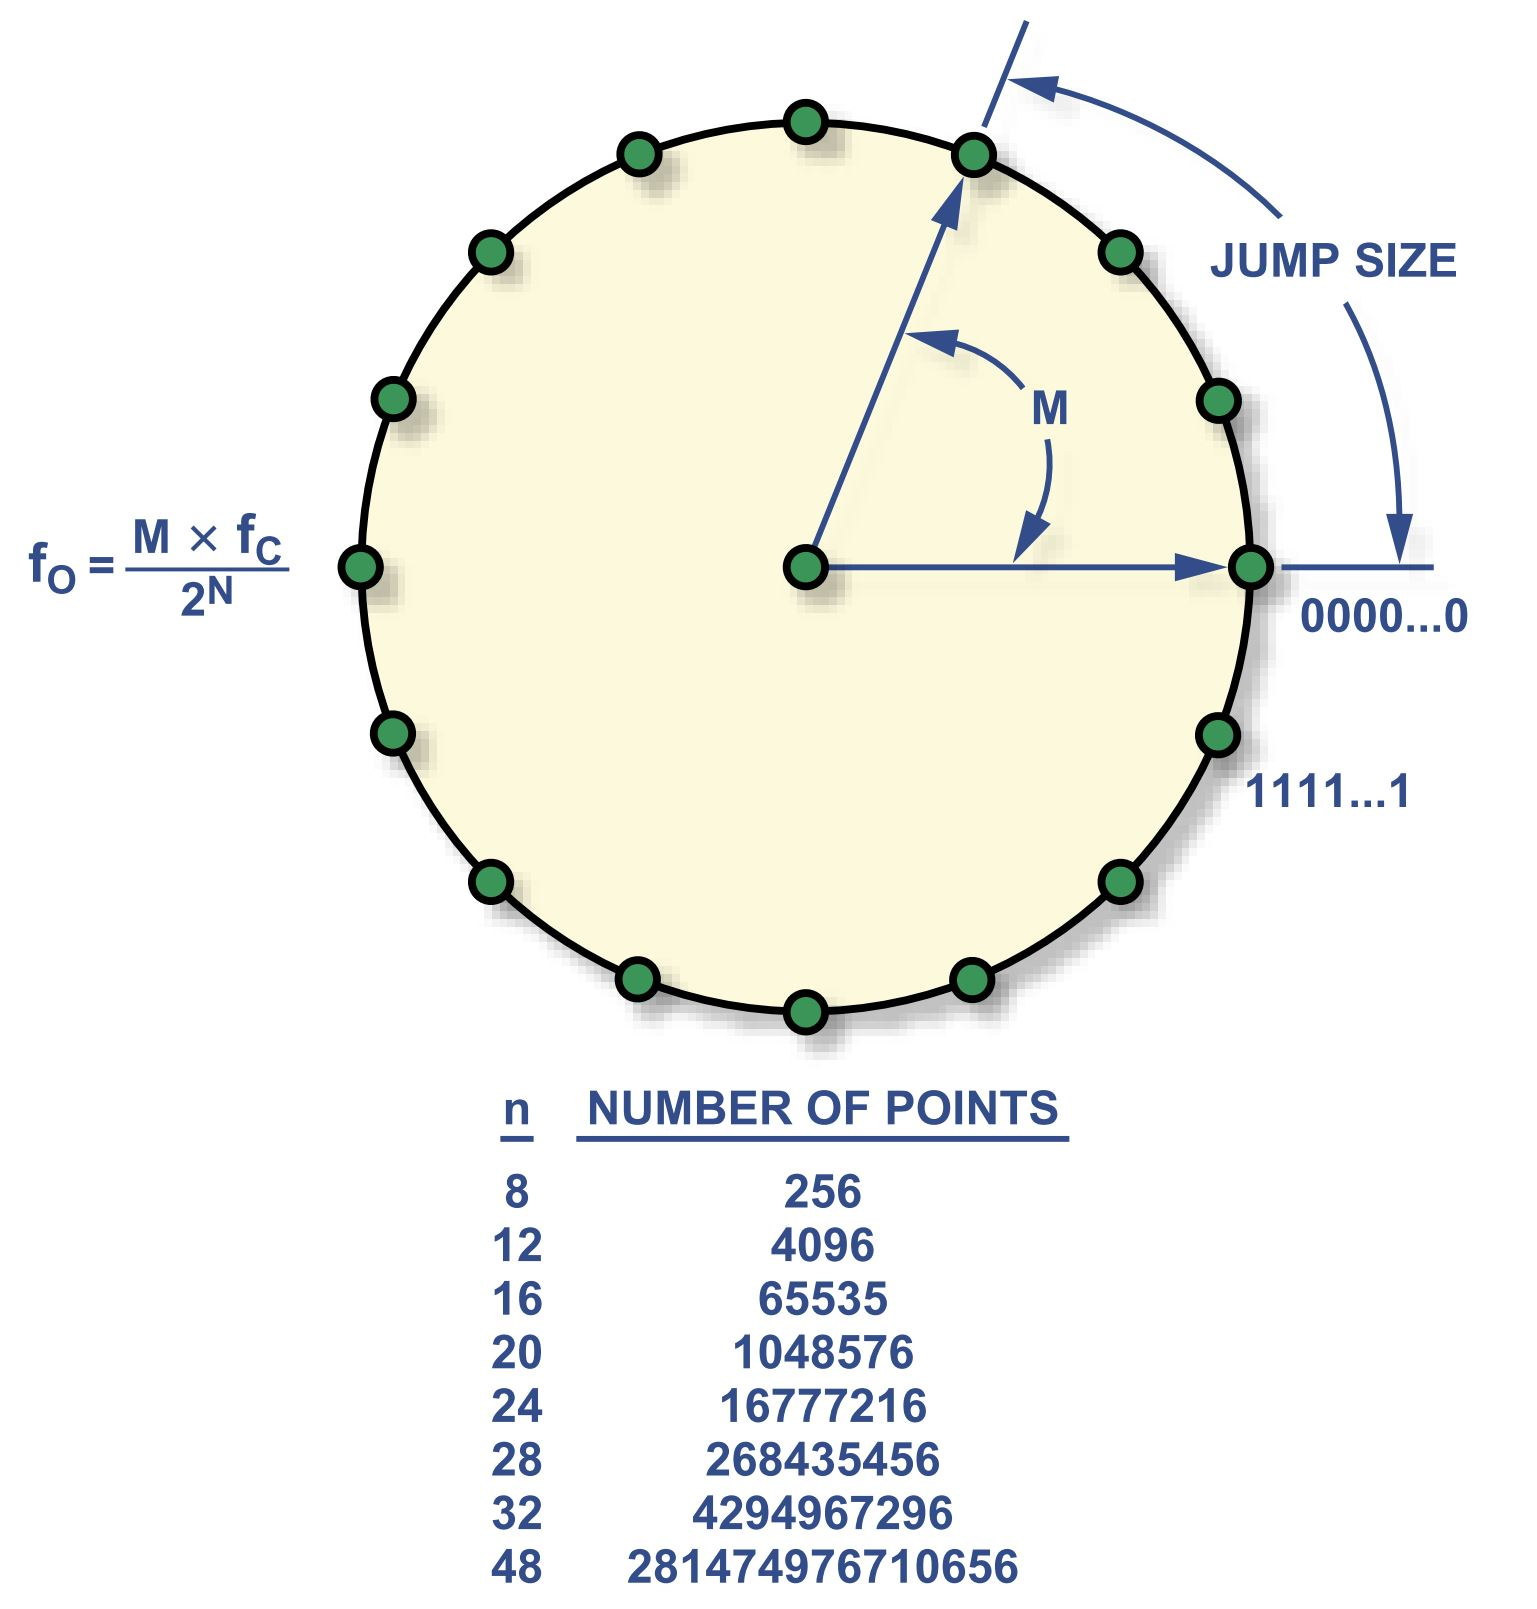
\includegraphics[width=\linewidth, height=80mm, keepaspectratio]{phase2amplitude-converter.jpg}
    \caption{Conversor de fase a amplitud, una \textit{look-up table} senoidal, extraído de \cite{murphy2004}.}
    \label{fig:look-up-table}
  \end{figure}

  Muchos DDS comerciales permiten controlar, además de la frecuencia, la fase y la amplitud de la onda generada y permiten realizar otras funciones como modulación de señales.

\end{standalone}
\end{document}
